% Main editable manuscript. Layout reference: BDX/Articolo_Neutroni/revtex.tex.
% APS/PRD reproduces the requested two-column layout; journal choice remains open.
\documentclass[10pt,aps,prd,amsmath,amssymb,superscriptaddress,twocolumn,nofootinbib,showpacs,showkeys,preprintnumbers,amsfonts,notitlepage,floatfix]{revtex4-2}
\usepackage[T1]{fontenc}
\usepackage[utf8]{inputenc}
\usepackage{graphicx}
\usepackage{booktabs}
\usepackage{xcolor}
\usepackage[hidelinks]{hyperref}
\usepackage{microtype}
\graphicspath{{figures/}}
\hypersetup{pdftitle={Preservation and modernisation of the GRAAL data and simulation framework},pdfsubject={Methods working draft; published-domain benchmark}}
\newcommand{\drafttodo}[1]{\par\smallskip\noindent{\small\color{red!55!black}\textbf{[TO COMPLETE: #1]}}\par\smallskip}
\newcommand{\reaction}{\gamma p\rightarrow\eta\pi^0p}
\begin{document}
\preprint{Working draft v0.2 --- Not for submission}
\title{Preservation and modernisation of the GRAAL data and simulation framework: validation through \texorpdfstring{$\eta\pi^0$}{eta pi0} photoproduction}
\author{Authors to be confirmed}
\affiliation{Affiliations to be confirmed}
\date{11 November 2026}
\begin{abstract}
The long-term scientific use of photoproduction archives requires the preservation of detector information, beam conditions, reconstruction software and simulation, together with the relationships between them. The GRAAL archive is particularly valuable because it combines tagged photons, controlled linear beam polarisation and broad detector coverage. We describe a preservation and modernisation programme connecting historical HBOOK data and the PAW analysis environment to ROOT, recovering Fortran algorithms within a C++/Python workflow, and migrating GEANT3-based simulation to Geant4. The reaction $\reaction$, reconstructed through its four-photon final state, provides a benchmark for the common reconstruction, boosted decision tree selection and polarisation analysis. Selected-event quality distributions and stored azimuthal fits illustrate the method; a restricted comparison with published GRAAL beam asymmetries tests the analysis interfaces in an existing measurement domain. Numerical software equivalence, calibrated detector response and observable-level validation are treated separately. The present draft documents these methods and diagnostic evidence, while the archival conversion audit, complete uncertainty treatment and quantitative performance validation remain to be completed. The resulting framework is intended to support future studies of unanalysed channels and more finely resolved measurements within the preserved archive.
\end{abstract}
\keywords{data preservation; photoproduction; polarised photon beams; ROOT; Geant4; multivariate analysis}
\maketitle
\raggedbottom
\noindent\textit{Draft status.} Figures use identified stored products, not a frozen publication campaign. The observable source explicitly marks final inference as suspended. Red completion notes identify missing publication evidence; the title states the intended validation scope, not a completed certification.

\section{Introduction}
Preserving experimental data means retaining the ability to ask new scientific questions of them. Event files alone do not retain the detector conditions, calibrations, selection logic and simulation assumptions needed to reconstruct a measurement. In high-energy and nuclear physics, preservation therefore extends from documentation and data formats to executable reconstruction and analysis chains \citep{DPHEP2023}.

The GRAAL photoproduction archive offers a strong case for this approach. Laser backscattering at the ESRF provided an energy-tagged photon beam with a controlled linear polarisation. For the ultraviolet sample described in Ref.~\citep{Ajaka2008}, the beam covered approximately 0.93--1.50 GeV and its polarisation ranged from about 0.60 to 0.96. The combination of beam information and detector coverage supports measurements of polarisation observables in exclusive reactions. Its value rests on these measured capabilities and on the surviving data, rather than on an assertion of uniqueness among laser-backscattering facilities.

The aim of this work is to preserve that capability while making the archive usable with current software and analysis methods. Three connected tasks are addressed: conversion of historical data representations, recovery and migration of reconstruction and analysis software, and migration of detector simulation. A fourth component, validation with an already measured reaction, connects the technical work to an observable. Figure~\ref{fig:preservation} summarises this strategy.

\begin{figure*}[t]
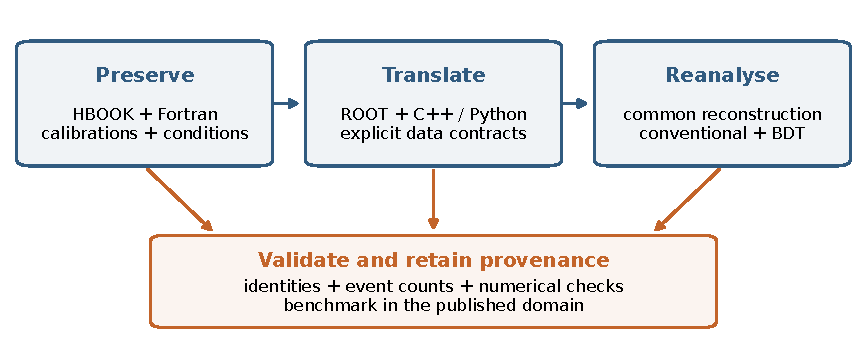
\includegraphics[width=\textwidth]{preservation_chain.pdf}
\caption{Preservation strategy. Historical inputs, source code and conditions remain traceable through translation and reanalysis. Validation links the layers through explicit checks; the diagram describes the strategy and does not imply that every audit or physical validation is complete.}
\label{fig:preservation}
\end{figure*}

We use $\reaction$, followed by $\eta,\pi^0\rightarrow\gamma\gamma$, as a benchmark. The final state tests photon pairing, recoil consistency, background rejection and the extraction of a beam asymmetry. Published GRAAL measurements provide a reference \citep{Ajaka2008}. The present methods study restricts its observable illustrations to that published domain. New energy intervals, an extended set of asymmetries, cross sections and analyses of additional channels are reserved for subsequent physics studies.

\drafttodo{Add the primary apparatus and polarimetry references; specify acquisition periods and archive coverage from a frozen publication inventory. Quantify the distinctive beam capabilities without claiming an unsupported experimental monopoly.}

\section{Preserving the data and their meaning}
\subsection{From HBOOK and PAW to ROOT}
The historical environment combined HBOOK ntuples with PAW-based analysis. HBOOK is the stored data representation; PAW is the analysis environment. Their modernisation requires both conversion of the records to ROOT \citep{Brun1997} and recovery of the definitions used to interpret those records. A branch name alone does not establish whether a quantity is measured, reconstructed or simulated, nor does it preserve its units, indexing conventions or detector status.

The modern chain reads detector-level records at the historical h70 boundary and produces preanalysed h80 records, followed by selected event products. Period-dependent particle-identification cuts remain explicit inputs. The preanalysis retains source identities and accounts for written and discarded events by run and beam state. Events lacking tagger information are counted as discarded rather than silently removed. This accounting is distinct from, and cannot substitute for, verification of the earlier HBOOK-to-ROOT conversion.

A complete archival conversion audit must connect each original file to its converted counterpart, record the conversion program and environment, and compare entry counts, types, array dimensions, units and representative values. Integer identifiers and flags require exact checks; numerical fields require declared tolerances justified by the stored precision. Missing values, overflow conventions and variable-length records must retain their meaning. Original files and historical results remain unchanged.

The current ROOT analysis boundary is operational, but the complete provenance linking the archived h70 files to historical PREAN builds and HBOOK conversion executions has not yet been established. Consequently, this draft does not claim a fully audited lossless conversion of the entire archive.

\subsection{From Fortran to C++ and Python}
The software migration preserves scientific definitions at component boundaries. Recovered Fortran sources provide reference implementations for detector response and reconstruction. C++ implements the modern detector and reconstruction components, while Python coordinates processing, configuration and analysis. The role of each language follows the component being preserved; a change of language is not itself a physics improvement.

Routine-level checks compare recovered and modern implementations on declared input domains. Particular attention is required for array indexing, initialisation, numerical precision, random-number use and detector identifiers. Agreement for a routine on controlled inputs establishes a local numerical result. It does not establish that the same historical configuration was used for every data period, or that a simulation reproduces measured detector response.

The preserved context therefore includes source snapshots, build options, calibration tables, period cuts, run manifests and model bundles. A publication release must bind these inputs to the resulting figures and analysis products. Table~\ref{tab:preservation} distinguishes the intended preservation products from the remaining evidence.

\begin{table*}[t]
\caption{Preservation boundaries and evidence required for the methods publication. Current implementation and planned validation are distinguished; the table is not a declaration that the full historical software has been ported.}
\label{tab:preservation}
\begin{ruledtabular}
\begin{tabular}{p{0.20\textwidth}p{0.32\textwidth}p{0.40\textwidth}}
Historical component & Modern representation or boundary & Validation evidence and present limit \\
\hline
HBOOK records; PAW analysis & ROOT records with explicit field definitions & ROOT processing available; original-to-converted file audit and historical runtime linkage remain open. \\
Fortran reconstruction and conditions & C++ components; Python orchestration; preserved cuts & Local numerical checks exist; source coverage and configuration equivalence require a frozen inventory. \\
GEANT3 simulation & Geant4 transport plus recovered response & Geometry and algorithm checks are separate from calibrated response, efficiency and acceptance validation. \\
Conventional event selection & Common reconstruction with an additional BDT gate & Selected-event controls available; independent efficiency, background and bias measurements remain required. \\
Published observables & Restricted comparison to Ajaka et al. & Diagnostic benchmark available; full uncertainties and correlations with the historical sample are unresolved. \\
\end{tabular}
\end{ruledtabular}
\end{table*}

\section{Preserving and modernising the simulation}
\subsection{Geometry, materials and transport}
The simulation migration starts from the preserved GEANT3 detector description \citep{GEANTManual} and connects it to Geant4 \citep{Agostinelli2003}. Geometry translation retains volume identities and placements needed to associate sensitive volumes with detector channels. The current baseline uses the GRAAL\_26 description, with recovered forward- and central-chamber paths. This baseline does not automatically represent every historical acquisition period.

Material interpretation is treated separately from geometric translation. Effective elemental parameters and mixtures in the historical description require explicit modern transport definitions. Source records remain preserved, while the composition and density used by Geant4 are recorded. Agreement of geometry names and positions is insufficient to establish agreement in material budget or interaction probability.

Target material, position and active length are period-dependent conditions. A reconstructed transverse vertex distribution is an acceptance- and resolution-dependent input, not an unfolded incident-beam profile. A deuterium detector geometry also does not supply a validated nuclear event generator. These distinctions keep detector configuration separate from reaction modelling.

\subsection{Response, reconstruction and event accounting}
Generated final-state four-vectors enter transport without the detector smearing used by the existing fast simulation, avoiding a second application of detector response. Generated-event identities and weights are retained through transport and selection, including events with no usable reconstructed candidate. Such events must remain in the appropriate efficiency denominator. Generator weights, photon exposure and branching fractions are distinct quantities.

Recovered response and reconstruction paths include calorimeter response, chamber tracking, central and forward associations, tagger information and the interface to the common analysis. Figure~\ref{fig:simulation} separates numerical equivalence from physical validation. Tests against original routines address the former. Independent detector data, period-specific conditions and observable closure address the latter.

\begin{figure*}[t]
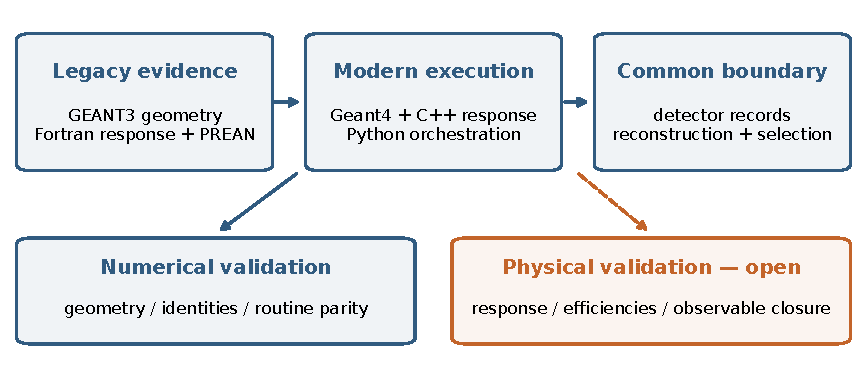
\includegraphics[width=\textwidth]{simulation_migration.pdf}
\caption{Simulation migration and its two validation levels. Preserved GEANT3/Fortran descriptions provide the reference for the modern transport and response chain. Numerical checks do not establish detector calibration. The physical-validation branch remains open; no Geant4 efficiency or resolution measurement is inferred from this schematic.}
\label{fig:simulation}
\end{figure*}

The present figures use archived-data analysis products. They are not evidence that the full Geant4 response has been calibrated, and they do not attribute the observed BDT-selected shapes to Geant4 training. The existing classifier samples use simplified detector response. A physically validated Geant4 production sample is a separate deliverable.

\drafttodo{Insert quantitative geometry/material comparisons, routine-parity coverage and independent detector-response plots from an identified simulation campaign. Freeze toolkit version, physics configuration, production cuts, detector thresholds and period conditions. Do not substitute a small technical pilot for efficiency validation.}

\section{Common reconstruction and multivariate selection}
\subsection{Benchmark event definition}
The reference topology contains four central photon candidates, one identified proton and no identified pion candidate. The established period-dependent particle-identification cuts are retained. The forward-track requirement depends on the proton polar angle: one forward charged track below $25^\circ$, and none above that boundary. Absence of an identified pion does not imply absence of every additional charged particle.

Four photons admit three disjoint pair partitions, each with two assignments to $\eta$ and $\pi^0$. The chosen assignment minimises
\begin{equation}
\chi^2_{\mathrm{pair}}=
\left(\frac{m_{\gamma\gamma}^{(\eta)}-m_\eta}{\sigma_\eta}\right)^2+
\left(\frac{m_{\gamma\gamma}^{(\pi^0)}-m_{\pi^0}}{\sigma_{\pi^0}}\right)^2.
\end{equation}
This is an assignment statistic, not a global constrained kinematic fit. The documented reconstruction uses relative mass scales of 0.08, $\chi^2_{\mathrm{pair}}<10$, a meson-energy consistency requirement and a recoil missing-mass window of $\pm0.06$ GeV around the proton mass. The latter quantity is formed from beam plus target minus the reconstructed mesons.

The conventional and BDT paths share these requirements. The BDT gate provides an additional selection, allowing its effect to be studied without changing the pairing or missing-mass definition. The model uses the same ordered 26-feature contract in training and inference. In particular, the feature formed from beam plus target minus the measured proton differs from the meson-based recoil missing mass used for event selection.

\subsection{Quality controls and the meaning of improved performance}
Figure~\ref{fig:masses} compares the stored meson-mass distributions after the conventional and BDT selections. Each distribution is normalised by its own event total, including flow bins. The comparison therefore shows selected shapes, not relative signal efficiencies. Figure~\ref{fig:quality} adds missing-mass, coplanarity and proton-angle controls. These are integrated ultraviolet diagnostics over 0.93--1.50 GeV; they do not display a new differential physics observable below the published asymmetry domain.

\begin{figure*}[t]
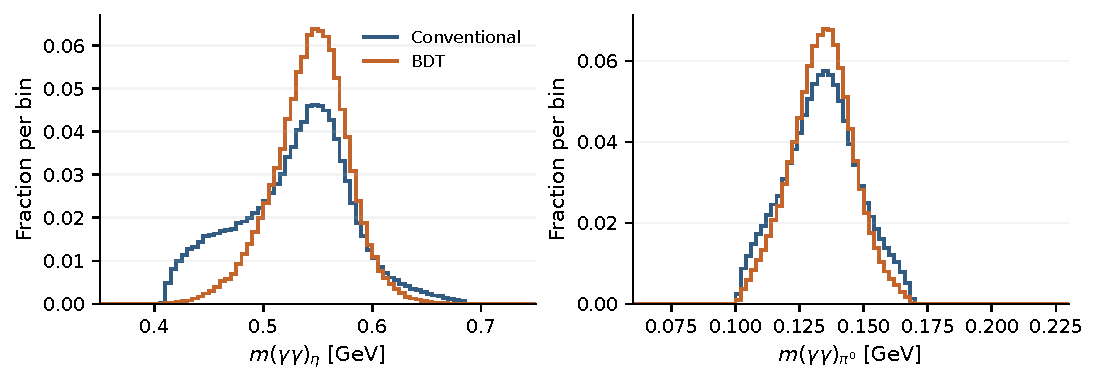
\includegraphics[width=\textwidth]{mass_quality.pdf}
\caption{Reconstructed two-photon masses after common conventional selection (blue) and additional BDT selection (orange). Stored ultraviolet quality-control histograms cover 0.93--1.50 GeV, with 257245 and 171599 selected entries, respectively. Each histogram is normalised independently, including flow bins. The mass-shape change is a selection diagnostic, not a measurement of intrinsic detector resolution or signal efficiency. No new mass fit is performed for this figure.}
\label{fig:masses}
\end{figure*}

\begin{figure*}[t]
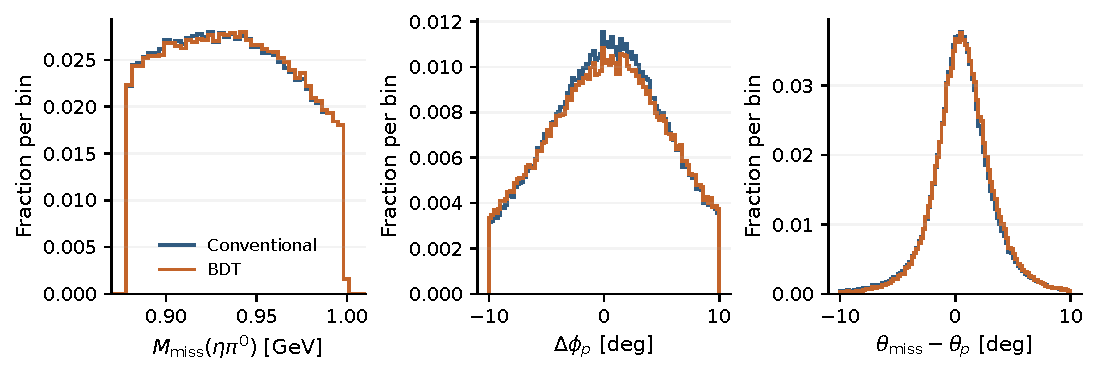
\includegraphics[width=\textwidth]{kinematic_quality.pdf}
\caption{Quality controls for the same samples and normalisation as Fig.~\ref{fig:masses}. The missing mass uses beam plus target minus the meson pair; its selection window has already been applied. Coplanarity is the wrapped difference $\phi_p-\phi_{\eta\pi^0}-180^\circ$. The angular residual compares the missing-proton and measured-proton directions. Angular underflow and overflow enter the normalisation even when outside the displayed range. These are selected-event distributions without acceptance or flux correction.}
\label{fig:quality}
\end{figure*}

The stored Gaussian diagnostics in the interval 0.50--0.60 GeV give $\eta$ widths of 33.2 MeV for the conventional selection and 29.5 MeV after the BDT gate. Their fit qualities, however, are $\chi^2/\mathrm{ndf}=579.7/17$ and $335.3/17$. A single Gaussian is thus not an adequate quantitative description of these distributions. The widths can describe a change in the selected peak shape, but cannot establish improved detector resolution. No resolution-gain percentage or significance is assigned to them.

A performance claim requires an independent test sample with identified signal and background, efficiencies at matched background rejection (or rejection at matched efficiency), and checks across relevant kinematics. Because mass-related quantities enter the selection, mass sculpting must be tested explicitly. Improved precision on an observable must also include selection bias and uncertainty, rather than follow from a narrower peak alone. Training, threshold choice and final testing require separate samples, keeping repeated versions of a generated event in the same partition.

\drafttodo{Add classifier implementation and reference, feature definitions, frozen model and threshold, independent performance curves, response or pull distributions, and observable closure. These figures are necessary before claiming better resolution or demonstrated BDT superiority; no synthetic performance curves are inserted.}

\section{Validation in the published measurement domain}
\subsection{Polarisation modulation and stored fits}
For perpendicular linear-polarisation states, beam-asymmetry information enters the azimuthal yields through a modulation proportional to $P_\gamma\Sigma$. The normalisation and sign convention must be retained through migration. With $y_V=N_V/F_V$ and $y_H=N_H/F_H$, the implemented ratio is
\begin{equation}
R(\phi)=\frac{y_V(\phi)-y_H(\phi)}{P_Hy_V(\phi)+P_Vy_H(\phi)}.
\label{eq:ratio}
\end{equation}
Here $F_V,F_H$ denote the corresponding photon exposures and $P_V,P_H$ the polarisation factors. Under the adopted azimuth convention and common-acceptance assumptions, the nominal model is $R(\phi)=\Sigma\cos(2\phi)$. Since Eq.~\eqref{eq:ratio} already removes the polarisation scale, its ordinate is not the raw product $P_\gamma\Sigma$.

Figure~\ref{fig:azimuth} shows stored ratio points and their fitted curves in $1.20<E_\gamma<1.30$ GeV. One mass bin in each projection is used, chosen by its position among the published reference points rather than by fit quality. The plotted cosine amplitude is the stored centre-fit amplitude, before correction for azimuthal-bin averaging. For the 12-bin fits shown, the extraction divides that amplitude by 0.9549 once when reporting $\Sigma$. Replotting does not apply an additional correction. Constant and sine terms are available as diagnostics; the displayed stored fits have both terms fixed to zero.

\begin{figure*}[t]
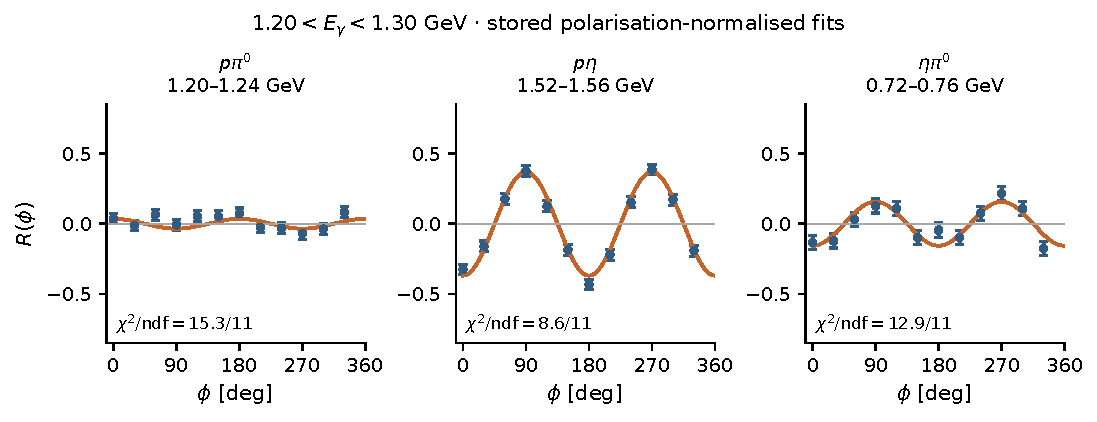
\includegraphics[width=\textwidth]{azimuthal_fits.pdf}
\caption{Examples of the beam-polarisation modulation analysis, restricted to the published Ajaka energy and mass domain. Points and errors are the stored polarisation-normalised ratio, Eq.~\eqref{eq:ratio}; curves reproduce the stored fit parameters without refitting. The three projections use the same underlying event sample and are correlated. The displayed $\chi^2$ values have been checked against the saved points. These provisional diagnostics are neither new-domain measurements nor raw $P_\gamma\Sigma$ plots.}
\label{fig:azimuth}
\end{figure*}

The analysis also provides a conditional-likelihood estimator retaining event exposure and polarisation information. Its intervals can be asymmetric; it is not rescaled by the ratio's finite-bin divisor. Comparisons between these estimators are methodological controls, not independent measurements of the same sample.

\subsection{Restricted comparison with Ajaka et al.}
Figure~\ref{fig:ajaka} compares the stored BDT-selected conditional-likelihood estimates with points digitised from Fig.~4 of Ref.~\citep{Ajaka2008}. Only one published energy interval and mass bins matching the published positions are shown. The modern 40 MeV bins are retained, avoiding a finer-bin physics result in this methods illustration. Digitised points are approximate representations of the published figure, not original numerical data supplied by its authors.

\begin{figure*}[t]
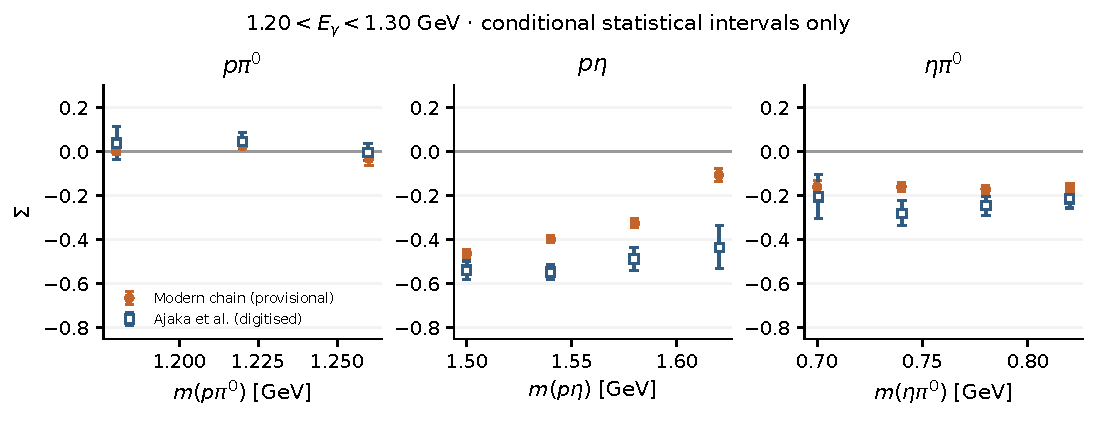
\includegraphics[width=\textwidth]{ajaka_benchmark.pdf}
\caption{Restricted published-domain benchmark in $1.20<E_\gamma<1.30$ GeV. Orange points show stored modern-chain conditional-likelihood estimates; open blue squares reproduce digitised Ajaka et al. points \citep{Ajaka2008}. Modern error bars are conditional statistical intervals only. Published asymmetric bars are retained as digitised; no digitisation uncertainty is inferred. The source campaign marks final inference as suspended. Full systematics, background treatment and inter-analysis covariance remain incomplete, so the figure does not establish quantitative closure or a final revised measurement.}
\label{fig:ajaka}
\end{figure*}

This comparison tests whether the preserved analysis can return to an existing observable domain while keeping conventions explicit. The $p\eta$ projection shows visible shifts relative to the digitised reference; their origin must be resolved before claiming benchmark closure. It does not constitute independent experimental confirmation: the new analysis can reuse events from the historical GRAAL sample, and the three mass projections are mutually correlated. Agreement or disagreement cannot be assigned a global significance by adding displayed errors in quadrature without the relevant covariance. The reference must not be used to tune the classifier or calibration towards a published answer.

The current source product marks final inference as suspended. Available systematic components do not constitute a complete uncertainty budget, and the stored benchmark does not by itself certify the background correction or photon-exposure treatment. This is why the figure is presented as diagnostic evidence within a working draft. A publication benchmark requires a frozen exposure policy, final background treatment, uncertainty propagation and an explicit accounting of shared data.

\drafttodo{Freeze the publication campaign and reference data. Complete exposure, background, polarisation and selection uncertainties, bias/coverage checks and covariance before claiming quantitative agreement.}

\section{Reproducibility and scientific reach}
The preservation product must remain usable beyond the benchmark reaction. A reproducible release should identify original and converted data, field definitions, code versions, detector conditions, simulation settings, classifier bundles and executable analysis configurations. Event accounting must retain rejected and unavailable outcomes as well as successful candidates. A test of re-execution should start from declared preserved inputs and reproduce the released validation products.

For this draft, each empirical figure is linked to a stored ROOT object or reference table. Input hashes, histogram normalisation, displayed energy and mass domains, fit conventions and plotting code are recorded alongside the manuscript. Figures are regenerated without modifying the historical scientific products. This provides figure-level traceability; it does not replace an archive-wide preservation audit or a reproducible release of the complete experiment software.

The same framework can support reactions not previously analysed, provided their topology, background, efficiency and polarisation response are validated. It may also allow previously measured channels to be revisited with finer kinematic binning or improved reconstruction. Finer bins represent a gain in reported granularity only when supported by statistics, migration control and systematic uncertainties. Improved physical resolution requires separate detector-response evidence. These prospective applications motivate preservation without pre-empting their physics results.

\section{Conclusions}
The proposed GRAAL methods study connects data preservation to renewed scientific use. Its core is the continuity from historical HBOOK records and Fortran software to ROOT-based C++/Python analysis, together with the migration of GEANT3 simulation to Geant4 and the retention of detector conditions and provenance. The $\eta\pi^0$ benchmark provides concrete selected-event controls and examples of the polarisation analysis within an already published domain.

The evidence assembled here illustrates the working analysis interfaces and the effects of selection. It does not yet establish a complete archival conversion audit, a fully calibrated Geant4 response or a quantitative gain in detector resolution and final observable precision. Completing those validations will determine the strength of the methods publication. A documented and reproducible framework can then support unanalysed channels and more detailed measurements of existing ones, with subsequent physics papers referring back to the preserved methodology.

\begin{acknowledgments}
\drafttodo{Confirm authorship, collaboration and institutional acknowledgments, funding, data/software availability, and the target journal's required disclosure of writing assistance.}
\end{acknowledgments}
\bibliographystyle{bst/apsrev4-2}
\bibliography{references}
\end{document}
